%----------------------------------------------------
\documentclass[
      11pt,
openright, 
  twoside,
]{book}
\usepackage[
    paperwidth=105mm,
    paperheight=148mm,
    inner=17mm,
    outer=12mm,
    top=15mm,
    bottom=20mm
]{geometry}
%----------------------------------------------------
\usepackage{tikz, lipsum}
\usetikzlibrary{calligraphy}


\usepackage{graphicx} % Required for inserting images
\usepackage[document]{ragged2e}
\usepackage{lettrine}
\usepackage{xstring}
\usepackage{color}
% \pagecolor{black}
% \color{white}

\newcommand{\myfleuron}{\vspace{5mm}% <-- additional space above
    {\centering
    \vspace{\fill}
    \tikz[baseline=-.68ex, scale=.65]
    {
    \pen (0,0) -- (30:.2);
    % \calligraphy[pen colour=white] (-1,0) to[out=30, in=210] ++(2,0)
    \calligraphy[] (-1,0) to[out=30, in=210] ++(2,0)([xshift=-1cm]30:.25)to[out=30, in=210] ++(2,0);}
    \par}
    \vspace{\fill}%
}

\usepackage{staves}
%----------------------------------------------------
\hyphenpenalty=5000
%----------------------------------------------------

%----------------------------------------------------
\newcommand{\quotepage}[1]{%
    \clearpage
    \thispagestyle{empty}
    \vspace*{\fill}
    \StrLeft{#1}{1}[\firstletter]%    
    \StrGobbleLeft{#1}{1}[\remainingtext]%    
    \lettrine[
        lines=2,%
        findent=2pt,%
        lhang=0.05,%
        lraise=0.15%
    ]{\firstletter}%
    {\remainingtext}%
    \vspace*{\fill}%
    \clearpage
}

\newcommand{\quotesmall}[1]{%
    \par
    \vspace*{\fill}
    \StrLeft{#1}{1}[\firstletter]%    
    \StrGobbleLeft{#1}{1}[\remainingtext]%    
    \lettrine[
        lines=2,%
        findent=2pt,%
        lhang=0.05,%
        lraise=0.15%
    ]{\firstletter}%
    {\remainingtext}% 
    % \vspace{5mm}
    \vspace*{\fill}
    \par
}    
%----------------------------------------------------
\renewcommand{\LettrineTextFont}{\textnormal}
%----------------------------------------------------

% \documentclass[a4paper]{article}
% \usepackage{pdfpages}

% \begin{document}

% \includepdf[
%     pages=-,
%     nup=2x2,
%     frame=true,
%     delta=0mm 0mm,
%     scale=0.95
% ]{input.pdf}

% \end{document}

%----------------------------------------------------

\title{ECA PhD Survival Advice}
\author{}
\date{}

\begin{document}

\pagestyle{empty}

\begin{center}
\vspace*{\fill}
\LARGE
ECA PhD\\Pocket Survival Advice\\
\vspace{10mm}
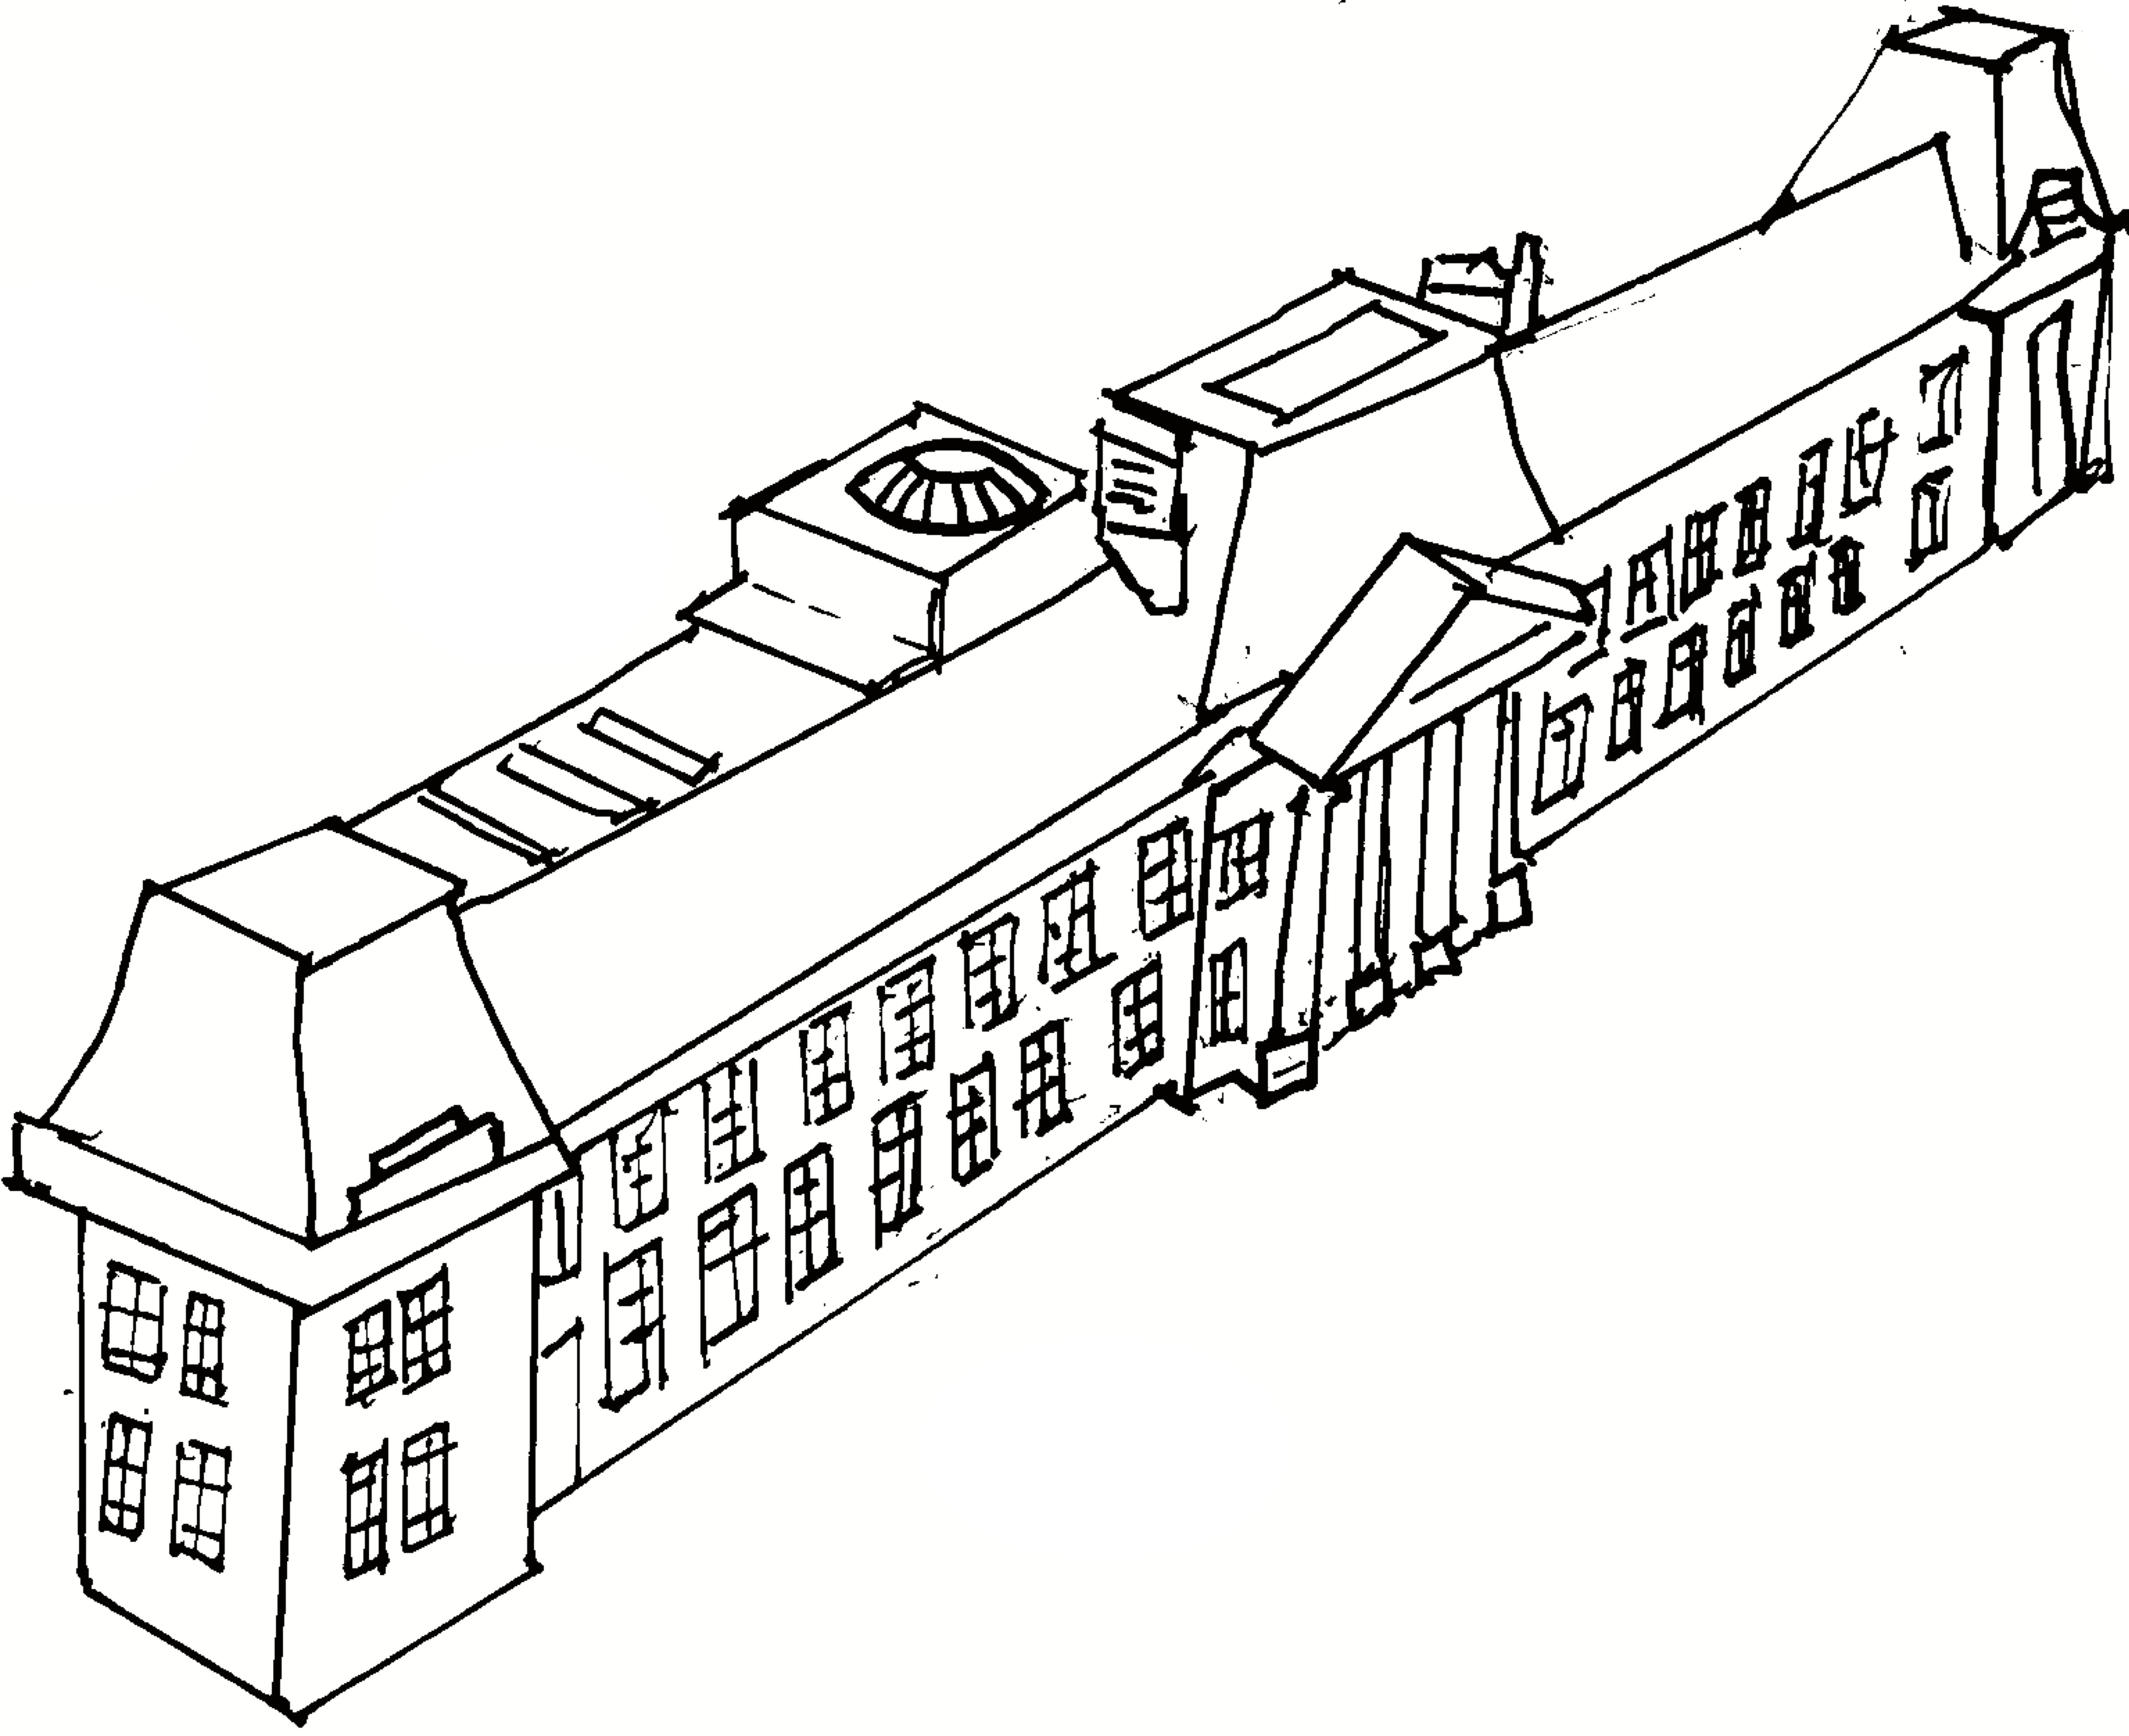
\includegraphics[width=.6\linewidth]{img/eca.png}
\vspace{10mm}

\normalsize
An unofficial companion\\to aid perseverance\\ during your time at\\Edinburgh College of Art
\vspace*{\fill}
\clearpage
\end{center}

\vspace*{\fill}
\quotesmall{The ECA Handbook knows all. Use it\newline liberally and generously.}
\myfleuron
\quotesmall{At some point halfway through, get some PhDs together, sit in a room and outline the chapters and their major section headings.}
\myfleuron
\quotesmall{Treat your PhD like a 9-to-5. Routine is the panacea for doubt.}
\vspace*{\fill}
\clearpage

\vspace*{\fill}
\quotesmall{Use a Reference Manager!}
\myfleuron
\quotesmall{Use every part of the animal. Everything you do, no matter how small, can probably have a place in your thesis.}
\myfleuron
\quotesmall{Every thesis chapter is conference paper waiting to happen. Also, a thesis chapter is just a conference paper that has been fished out of the rubbish and then had the ugly parts painted over.}

\quotepage{Talk to people! In your first year you will probably be taking a class or two,  going to some lectures, finding your feet, finding out where things are and building relationships. Don't put off getting in touch with people. If you think you'll need someone’s help or assistance in 2 years, start building those relationships now. They take time.}

\quotepage{Take Vitamin D during the winter. This is Scotland for crying out loud.}


\quotepage{Get a certificate for everything. If you attended a big conference, or if you were invited to speak for five minutes during a lecturer, get the organiser to write a letter and sign it. When someone asks, ``what have you been doing,'' those certificates will come in handy.}

\clearpage
\quotesmall{Submit your writing to transparent peer-reviewed journals and conferences. You might not have the work accepted, but you will get 3 to 5 academics giving you feedback for free.}
\myfleuron
\quotesmall{When it comes down to it, a thesis will just be a ``thing you did.'' It does not define you.}
\myfleuron
\quotesmall{Write the text you wish you had when you started researching your thesis.}
\clearpage
\vspace*{\fill}

\quotesmall{Don't be afraid to admit you have wasted time, but document it as a warning for others.}
\myfleuron  
\centering
\footnotesize
\textsc{Hic Sunt Dracones}\\
\myfleuron  
\includegraphics[width=0.5\linewidth]{img/scholar.png}
\vspace*{\fill}

\clearpage
\normalsize
\raggedright

\quotepage{Take the first few months to settle in. Figure out what software you want to use (e.g. Zotero / Overleaf / \&c.); how you will organise your readings; what you care about and what your priorities will be; how you want to manage your relationship with your supervisor; how you want to structure your weeks (e.g. I work at home on Fridays, and normally in the office every afternoon). Giving yourself the time to figure these things out early will be useful in the long run – questions like these are not a waste of time!! Do not feel like you have to jump into the meat of your thesis immediately.}

\vspace*{\fill}
\quotesmall{You need a community bigger than the University. If you have any hobbies, try attending workshops/events/classes that would allow you to meet people outside of the campus. Conferences are also a good place to meet new people (in academia), especially people researching similar topics (so they speak 'your language'!). }
\vspace*{\fill}
\centering

\includegraphics[width=0.35\linewidth]{img/rowan.png}
\vspace*{\fill}

\raggedright
\quotepage{Don't sit at your desk and keep trying to work if you feel you are banging your head against the wall. If you reach a point in the day where you feel like you aren't getting anything done, go home and do the washing and buy a snack on the way. There's no point burning yourself out just because you feel like you should be working.}

% \vspace*{\fill}
\centering
\textsc{Dans le doute, pause café}\\
\vspace{10mm}

\raggedleft
--- Le Mans, Traditional
\vspace*{\fill}

\raggedright

\quotepage{There is no single way of doing a PhD. Just because others are on a different timeline to you, doesn’t mean you’re doing it wrong. Building on this, don’t simply do everything your supervisor says. Their way of doing a PhD isn’t the only way, so stay in open dialogue with them. If things are moving too fast, or too slow, tell them. If they suggest something you’re not 100\% convinced by, speak to your second supervisor or your fellow students. Academia is changing, and not all supervisors seem to be aware of it. Finally, this is YOUR PhD, not theirs!}

\vspace*{\fill}
\quotesmall{If you use a lot of primary source material in your research, don’t be afraid to jump right in. The sources may likely be the backbone of your argument and also might dictate what secondary source reading you need to do. So start with the exciting stuff, go to collections, get out there! Have fun looking at what you love.}
\myfleuron
\quotesmall{A major incident/unexpected personal event which severely/permanently alters your life can happen and affect your studies despite your best effort in planning and preparing for the entirety of PhD studies.}
\vspace*{\fill}


\vspace*{\fill}


\raggedright
\normalsize

\quotepage{Be kind to yourself and take breaks. It doesn’t feel like it now, but you do actually have time to take them. Burning out and getting sick can both sneak up on you and can take even more time to recover from. If you aren’t feeling productive or if you are pushing yourself harder than usual to focus, take the rest of the day to rest or go do something separate from the PhD.}

\quotepage{Someone told me that I should see myself as my own project manager, and I have found this SO useful. Every supervisor is different, but seeing your thesis as your own project will help you lead the way and get the most out of your time with your supervisor. Propose your own deadlines, think about what portion of your thesis makes most sense for you to work on first, reflect on what skills you are missing and how/when to develop them, send your supervisor short agendas ahead of your meeting to direct the conversation (I keep a draft email in my Outlook at all times with questions/topics to discuss with my supervisor. I write up our agendas based on this), write down your own concerns when you send a draft in for feedback. Again, it depends on your supervisor, but I found that taking the lead helped them help me. }
\vspace*{\fill}
\quotesmall{Diversify your working space if it helps you. I love the National Library of Scotland (you can make a reader's card for free, it's a 10-minute walk from ECA, and a great space for strike periods). I also regularly go to the Main Library (5th floor is for postgrads) and to Cafes. }
\vspace*{\fill}
\centering

\includegraphics[width=\linewidth]{img/calton.png}
\vspace*{\fill}
\clearpage

\raggedright
\quotepage{People will tell you that you should always be writing (i.e. not to leave it until the end), but this can sound really daunting. Writing can take MANY different forms. I have found it useful to: summarise readings in a few sentences after I read them, including if I found them good/bad and/or helpful (this helps remember the main arguments / remain analytical); jot down arguments and other thoughts as you think them (I keep a document dedicated to this type of free-thinking); write down very rough structures for chapters or subchapters regularly (I tend to dedicate 1--2 hours to this on Friday mornings, as a way to reflect on the week. This also helps me figure out what to read/do next. By structures, I often mean a list of bullet points). All of these are forms of writing! You do not need to be writing big chunks of text at all times! But these little bits will help you immensely when it is time to write up a whole chapter!}

\quotepage{Everyone is different but I recommend ALWAYS starting with structure before writing. What are the main things you want to say in this section? What is the order that makes the most sense? I always start off with a very thin structure, and then fill it up slowly (i.e. what primary/secondary sources will help me make this argument).}

\quotesmall{Not every day has to be productive. Don't beat yourself up if not much gets done from time to time. That would be the case if you had a normal 9--5 job, and there is no reason for it not to be the case with your PhD.}
\myfleuron
\quotesmall{My supervisor told me to romanticise your PhD. This is a really special and exciting time in your life, so don't hesitate to act like it. Enjoy the gloomy workdays, the silent libraries, the cafe work mornings, \&c. }
\myfleuron
\quotesmall{It's totally fine if you can't make friends yet and don't force yourself to go to gatherings / parties that you don't really enjoy.}
\clearpage
\quotesmall{MAKE FULL USE of the PRE grant (£500 each academic year until the writing up year for each student) for conferences and field work.}
\myfleuron
\quotesmall{There is no such thing as a ``normal'' PhD. There is no ``correct'' way to work. There is no ``right'' number of conferences or publications to aim for. There is no ``right'' number of words you should have written at each stage of the project.}
\myfleuron
\quotesmall{Find a working routine that works for you and do not panic if you feel are not where you should be with your project. It is a long-term piece of work, and you will take time to find your feet and to figure out exactly what the project is. Enjoy the process and the freedom that comes with that.}
\clearpage
\quotesmall{Come into campus and speak to the older students. They’ll be far more helpful in offering advice than the university! If you’re working by distance, send them an email. Doing a PhD in the UK isn’t easy, and it’s getting harder. Nobody is holding your hand through it, but that doesn’t mean help isn’t out there.}
\myfleuron
\quotesmall{Make the best of use of the university’s services (counselling \& mentoring from health \& wellbeing) for professional psychological support which friends at some point can’t provide \& when you’re far away from family.}
\quotepage{Building some form of routine early will help you later. You don’t have to treat it like a nine till five if you’re efficient with your time, but having a baseline is good. And if you get stuck somewhere, don’t fixate --- you’ll probably have a few other things to explore, while you think it over. }
\vspace*{\fill}
\quotesmall{Try not to compare progress on your thesis with fellow PhD students. Everyone’s project is so different that progress differs greatly between them. It’s really tough to do and I still remind myself of this years later, but as long as you and your supervisors are happy with your progress that is all that matters.}
\vspace*{\fill}
% \clearpage
% \vspace*{\fill}
\centering

\includegraphics[width=0.45\linewidth]{img/uoe.png}
\vspace*{\fill}
\end{document}
